% Model các cái này ra:
% Rating, efficiency, capacity, loa, cost, lifetime
% e the bay gio la sau khi tim duoc cai thiet bi dien roi ay, se thu duoc nhung gia tri nao? (kieu la tong kwh, cai continuous cao nhat (la khi nhieu appliances dung cung mot luc), va cai instantaneous dung ko))

When installing a battery storage system, we need to determine the types of batteries being installed in the home and the number of batteries installed. In the following equation:
\begin{equation}
    N_b = \frac{P_d \times L_a}{C_a}
\end{equation}

, we will be able to find the number of batteries needed in our system. However, the equation does not take into account the different types of batteries than can be presented in our system. It is therefore necessary to explore different types of batteries, their specifications in order to determine their strengths and weaknesses after installing in our photovoltaic system.

With that in mind, we need to analyse the specifications of different batteries. There are many brands and types of battery chemistry commercially available. Therefore, before installing the batteries in our photovoltaic system, we need to consider our choices:
\begin{enumerate}
    \item Lead-acid batteries
\end{enumerate}
Lead-acid battery is the most popular and reliable chemistry used in a PV storage system, as it has been around since the 19th century. The stored chemical potential energy in the battery can be converted to electrical energy through the following reaction:

$$\mathrm{Pb}+\mathrm{PbO}_{2}+2 \mathrm{H}_{2} \mathrm{SO}_{4} \rightarrow 2 \mathrm{PbSO}_{4}+2 \mathrm{H}_{2} \mathrm{O}$$
$$
E^{0}=2.041 V
$$
, in which the voltage produced from the reaction is $2V$.\cite{wiki:lead_acid_battery}

There are many different lead-acid batteries available for solar arrays, and these batteries offer different solutions to our energy needs. After researching online for lead-acid batteries, here are our choices when modeling the 

\begin{enumerate}[resume]
    \item Lithium-ion batteries (primarily lithium cobalt oxide)
\end{enumerate}
Lithium-ion batteries, despite being more expensive than their lead-acid counterpart, are more efficient and allow more depth of discharge than their counterpart, thus being more cost-effective in the long run. Via separating the lithium ions from the electrons via an electrolyte, the electron therefore can be directed through a circuit in order to discharge the chemical potential energy inside.\cite{wiki:li_ion_battery} \\

\begin{enumerate}[resume]
    \item Lithium iron phosphate (LFP) batteries
\end{enumerate}
LFP battery is a type of lithium-ion battery that uses lithium iron phosphate instead of lithium cobalt oxide as cathode material. While the energy density and voltage of this type of battery is lower than that of traditional lithium-ion battery, it is generally safer, cheaper , has higher discharge rate and has more life cycle than that of lithium-ion does.\cite{wiki:lfp_battery}\\ 

With all of that in mind, we decided to choose 10 batteries, with 4 being lead-acid batteries, 4 being lithium-ion batteries and 2 being lithium iron phosphate batteries. This is because we need to test a variety of battery in order to find the most optimal choice between different batteries.
\newpage
\paperwidth=\pdfpageheight
\paperheight=\pdfpagewidth
\pdfpageheight=\paperheight
\pdfpagewidth=\paperwidth
\headwidth=\textheight
\begingroup 
\vsize=\textwidth
\hsize=\textheight
\begin{figure}[H]
    \centering
    \textbf{Table 4:} Specifications of multiple batteries
    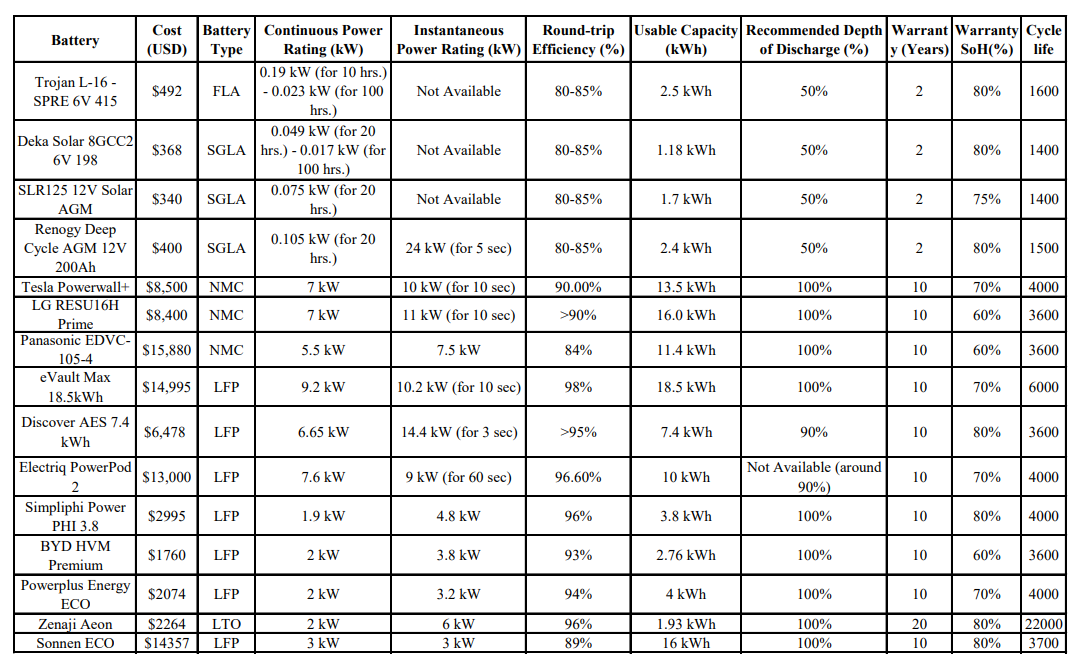
\includegraphics[scale=1.25]{src/aa.png}
\end{figure}

\endgroup
\newpage
\paperwidth=\pdfpageheight
\paperheight=\pdfpagewidth
\pdfpageheight=\paperheight
\pdfpagewidth=\paperwidth
\headwidth=\textwidth

\begin{comment}
\newgeometry{a3paper}
\paperwidth=\pdfpageheight
\paperheight=\pdfpagewidth
\pdfpageheight=\paperheight
\pdfpagewidth=\paperwidth
\headwidth=\textheight
\begingroup 
\vsize=\textwidth
\hsize=\textheight
% Table generated by Excel2LaTeX from sheet 'Sheet1'
\begin{table}[H]
  \centering
  \caption{Currently available battery models}
    \begin{tabular}{|p{6.865em}|p{3.32em}|l|p{7.725em}|p{7.635em}|l|p{6.225em}|l|l|l|l|}
    \toprule
    \textbf{Battery} & \textbf{Cost (USD)} & \multicolumn{1}{p{3.09em}|}{\textbf{Battery Type}} & \textbf{Continuous Power Rating (kW)} & \textbf{Instantaneous Power Rating (kW)} & \multicolumn{1}{p{5.865em}|}{\textbf{Round-trip Efficiency (\%)}} & \textbf{Usable Capacity (kWh)} & \multicolumn{1}{p{8.275em}|}{\textbf{Recommended Depth of Discharge (\%)}} & \multicolumn{1}{p{4.045em}|}{\textbf{Warranty (Years)}} & \multicolumn{1}{p{4.045em}|}{\textbf{Warranty SoH(\%)}} & \multicolumn{1}{p{4.045em}|}{\textbf{Cycle life}} \\
    \midrule
    Trojan L-16 -SPRE 6V 415 & \multicolumn{1}{l|}{\$492 } & \multicolumn{1}{p{3.09em}|}{FLA} & 0.19 kW (for 10 hrs.) - 0.023 kW (for 100 hrs.) & Not Available & \multicolumn{1}{p{5.865em}|}{80-85\%} & 2.5 kWh & 50\%  & 2     & 80\%  & 1600 \\
    \midrule
    Deka Solar 8GCC2 6V 198 & \multicolumn{1}{l|}{\$368 } & \multicolumn{1}{p{3.09em}|}{SGLA} & 0.049 kW (for 20 hrs.) - 0.017 kW (for 100 hrs.) & Not Available & \multicolumn{1}{p{5.865em}|}{80-85\%} & 1.18 kWh & 50\%  & 2     & 80\%  & 1400 \\
    \midrule
    SLR125 12V Solar AGM & \multicolumn{1}{l|}{\$340 } & \multicolumn{1}{p{3.09em}|}{SGLA} & 0.075 kW (for 20 hrs.) & Not Available & \multicolumn{1}{p{5.865em}|}{80-85\%} & 1.7 kWh & 50\%  & 2     & 75\%  & 1400 \\
    \midrule
    Renogy Deep Cycle AGM 12V 200Ah & \multicolumn{1}{l|}{\$400 } & \multicolumn{1}{p{3.09em}|}{SGLA} & 0.105 kW (for 20 hrs.) & 24 kW (for 5 sec) & \multicolumn{1}{p{5.865em}|}{80-85\%} & 2.4 kWh & 50\%  & 2     & 80\%  & 1500 \\
    \midrule
    Tesla Powerwall+ & \multicolumn{1}{l|}{\$8,500 } & \multicolumn{1}{p{3.09em}|}{NMC} & 7 kW  & 10 kW (for 10 sec) & 90.00\% & 13.5 kWh & 100\% & 10    & 70\%  & 4000 \\
    \midrule
    LG RESU16H Prime & \multicolumn{1}{l|}{\$8,400 } & \multicolumn{1}{p{3.09em}|}{NMC} & 7 kW  & 11 kW (for 10 sec) & \multicolumn{1}{p{5.865em}|}{>90\%} & 16.0 kWh & 100\% & 10    & 60\%  & 3600 \\
    \midrule
    Panasonic EDVC-105-4 & \multicolumn{1}{l|}{\$15,880 } & \multicolumn{1}{p{3.09em}|}{NMC} & 5.5 kW & 7.5 kW & 84\%  & 11.4 kWh & 100\% & 10    & 60\%  & 3600 \\
    \midrule
    eVault Max 18.5kWh & \multicolumn{1}{l|}{\$14,995 } & \multicolumn{1}{p{3.09em}|}{LFP} & 9.2 kW & 10.2 kW (for 10 sec) & 98\%  & 18.5 kWh & 100\% & 10    & 70\%  & 6000 \\
    \midrule
    Discover AES 7.4 kWh & \multicolumn{1}{l|}{\$6,478 } & LFP   & \multicolumn{1}{l|}{6.65 kW} & \multicolumn{1}{l|}{14.4 kW (for 3 sec)} & >95\% & \multicolumn{1}{l|}{7.4 kWh} & 90\%  & 10    & 80\%  & 3600 \\
    \midrule
    Electriq PowerPod 2 & \multicolumn{1}{l|}{\$13,000 } & \multicolumn{1}{p{3.09em}|}{LFP} & 7.6 kW & 9 kW (for 60 sec) & 96.60\% & 10 kWh & \multicolumn{1}{p{8.275em}|}{Not Available (around 90\%)} & 10    & 70\%  & 4000 \\
    \midrule
    Simpliphi Power PHI 3.8 & \$2995 &       & 1.9 kW & 4.8 kW & 96\%  & 3.8 kWh & 100\% & 10    & 80\%  & 4000 \\
    \midrule
    BYD HVM Premium & \$1760 &       & 2 kW  & 3.8 kW & 93\%  & 2.76 kWh & 100\% & 10    & 60\%  & 3600 \\
    \midrule
    Powerplus Energy ECO & \$2074 & \multicolumn{1}{p{3.09em}|}{Li-ion} & 2 kW  & 3.2 kW & 94\%  & 4 kWh & 100\% & 10    & 70\%  & 4000 \\
    \midrule
    Zenaji Aeon & \$2264 & \multicolumn{1}{p{3.09em}|}{LTO} & 2 kW  & 6 kW  & 96\%  & 1.93 kWh & 100\% & 20    & 80\%  & 22000 \\
    \midrule
    Sonnen ECO & \$14357 &       & 3 kW  & 3 kW  & 89\%  & 16 kWh & 100\% & 10    & 80\%  & 3700 \\
    \bottomrule
    \end{tabular}%
  \label{tab:addlabel}%
\end{table}%
\endgroup
\newpage
\paperwidth=\pdfpageheight
\paperheight=\pdfpagewidth
\pdfpageheight=\paperheight
\pdfpagewidth=\paperwidth
\headwidth=\textwidth
\restoregeometry
\end{comment}
asdfasdf